\subsubsection{User table}
Tabellen indeholder data om brugerne i systemet. Tabellen giver også mulighed for brugeren at tilgå dronerne, events og de gemte ruter i systemet, via tabellens Foring keys.
\vspace{-5pt}
\begin{figure}[H]
	\centering
	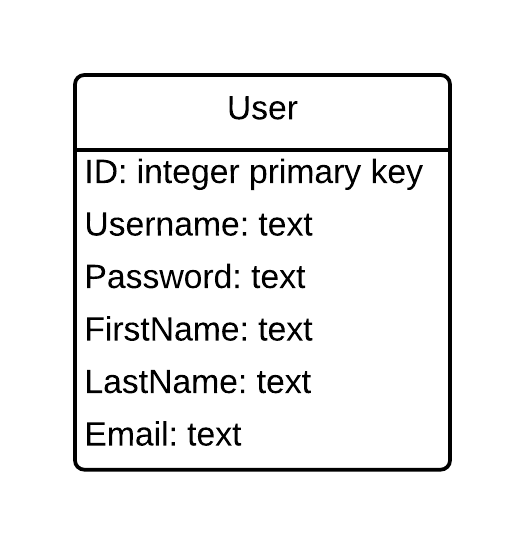
\includegraphics[width=0.5\textwidth]{Billeder/database/UserTabel.png}
	\vspace{-5pt}
	\caption{User table}
	\label{fig:user_table}
\end{figure}

\begin{table}[H]
\begin{tabular}{| p{3cm}| p{11.5cm}|}
\hline

Formål	 							& Holde data om brugeren i systemet, samt tjekke om brugeren eksterre ved forsøg på login.\\\hline
Forbindelser						& Tabellen har en Foring key til Helper User Drone og Helper User Event hjælpe tabellerne.\\\hline
Attributter						& \begin{itemize}
												\item ID: Primary key.
												\item Username: Brugernavnet til systemet. Max length: 50 char
												\item Password: Brugerens kode. Max length: 50 char
												\item FirstName: Brugers fornavn. Max length: 50 char
												\item LastName: Brugerens efternavn. Max length: 50 char
												\item Email: Brugerens email adresse.
											\end{itemize} \\\hline 
\end{tabular}
\caption{User table}
\label{tab:user_table}
\end{table}